% Created 2016-06-02 四 22:50
\documentclass[xcolor=svgnames,presentation]{beamer}
\usepackage[utf8]{inputenc}
\usepackage[T1]{fontenc}
\usepackage{fixltx2e}
\usepackage{graphicx}
\usepackage{longtable}
\usepackage{float}
\usepackage{wrapfig}
\usepackage{soul}
\usepackage{textcomp}
\usepackage{marvosym}
\usepackage{wasysym}
\usepackage{latexsym}
\usepackage{amssymb}
\usepackage{hyperref}
\tolerance=1000
\usepackage{minted}
\usecolortheme[named=FireBrick]{structure}\setbeamercovered{transparent}\setbeamertemplate{caption}[numbered]\setbeamertemplate{blocks}[rounded][shadow=true] \usetheme{Darmstadt}\date{\today} \usepackage{tikz}\usepackage{xeCJK}\usepackage{amsmath}\setmainfont{Times New Roman}\setCJKmainfont[BoldFont={Adobe Heiti Std},ItalicFont={Adobe Fangsong Std}]{Adobe Heiti Std}\setCJKsansfont{Adobe Heiti Std}\setCJKmonofont{Adobe Fangsong Std}\usepackage{verbatim}\graphicspath{{figures/}} \definecolor{lstbgcolor}{rgb}{0.9,0.9,0.9} \usepackage{listings}\usepackage{minted} \usepackage{fancyvrb}\usepackage{xcolor}\lstset{escapeinside=`',frameround=ftft,language=C,breaklines=true,keywordstyle=\color{blue!70},commentstyle=\color{red!50!green!50!blue!50},frame=shadowbox,backgroundcolor=\color{yellow!20},rulesepcolor=\color{red!20!green!20!blue!20}}
\usemintedstyle{default}
\providecommand{\alert}[1]{\textbf{#1}}

\title{第10讲 网络资源共享}
\author{王晓庆}
\date{\today}
\hypersetup{
  pdfkeywords={},
  pdfsubject={},
  pdfcreator={Emacs Org-mode version 7.9.3f}}

\institute{wangxiaoqing@outlook.com}
\begin{document}

\maketitle

\begin{frame}
\frametitle{Outline}
\setcounter{tocdepth}{1}
\tableofcontents
\end{frame}
\section{NFS服务}
\label{sec-1}
\begin{frame}
\frametitle{NFS工作原理(1)}
\label{sec-1-1}
\begin{itemize}

\item 在NFS服务器上设置共享目录,客户端可以将该共享目录挂载到本地挂载点,然后就可以像本地目录一样使用。\\
\label{sec-1-1-1}%
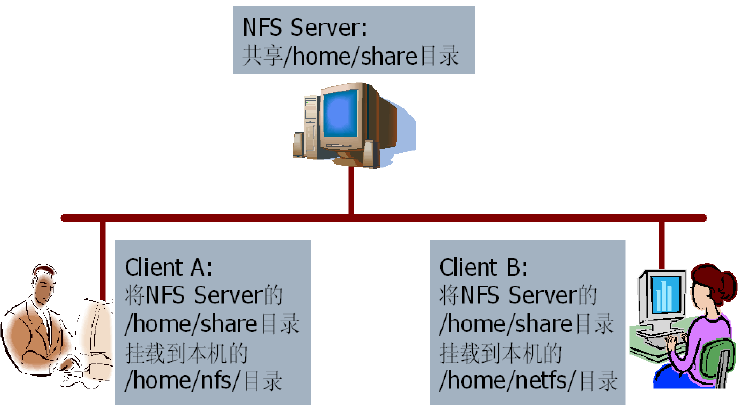
\includegraphics[width=.9\linewidth]{img/nfs.png}
\end{itemize} % ends low level
\end{frame}
\begin{frame}
\frametitle{NFS工作原理(2)}
\label{sec-1-2}
\begin{itemize}

\item NFS可实现文件共享,但要借助于RPC协议实现数据传输,要使用NFS,客户端和服务器端都需要启动RPC。
\label{sec-1-2-1}%

\item 对于NFS,RPC最主要的功能是指定每个NFS功能所对应的端口号,并且告知客户端,让客户端可以链接到正确的端口。
\label{sec-1-2-2}%
\begin{enumerate}
\item 服务器启动NFS时随机取用多个端口,并主动向RPC注册各功能端口
\item RPC使用111端口监听客户端请求
\item 客户端向服务器RPC(111端口)发出NFS文件访问功能的查询请求
\item RPC将NFS注册的守护进程端口号告知客户端
\item 客户端根据得到的端口号直接与NFS守护进程通信
\end{enumerate}
\end{itemize} % ends low level
\end{frame}
\begin{frame}
\frametitle{NFS必需的系统守护进程}
\label{sec-1-3}
\begin{itemize}

\item rpc.nfsd
\label{sec-1-3-1}%
\begin{itemize}

\item 基本的NFS守护进程,主要功能是管理客户端是否能够登录服务器
\label{sec-1-3-1-1}%
\end{itemize} % ends low level

\item rpc.mountd
\label{sec-1-3-2}%
\begin{itemize}

\item RPC挂载守护进程,主要功能是管理NFS文件系统。当客户端通过rpc.nfsd成功登录NFS服务器后,必须通过文件使用权限的验证(由rpc.mountd读取NFS配置文件来确认客户端权限),才能使用NFS服务器提供的文件
\label{sec-1-3-2-1}%
\end{itemize} % ends low level

\item portmap
\label{sec-1-3-3}%
\begin{itemize}

\item 主要用于端口映射,当客户端尝试连接并使用RPC所管理的服务(如NFS)时,portmap将所管理服务的对应端口号提供给客户端,从而使客户端可以通过该端口向服务器发出请求。
\label{sec-1-3-3-1}%
\end{itemize} % ends low level
\end{itemize} % ends low level
\end{frame}
\begin{frame}[fragile]
\frametitle{安装NFS服务器}
\label{sec-1-4}
\begin{itemize}

\item 正常允许NFS服务需要安装以下两个软件包
\label{sec-1-4-1}%
\begin{itemize}

\item nfs-utils(NFS主程序),默认已安装
\label{sec-1-4-1-1}%

\item portmap(RPC主程序),默认已安装
\label{sec-1-4-1-2}%
\end{itemize} % ends low level

\item 启动NFS(注意顺序!)\\
\label{sec-1-4-2}%
\begin{minted}[]{bash}
service portmap start #客户端也要启动portmap服务!
service nfs start
rpcinfo -p            #打印rpc注册端口信息
\end{minted}

\item 停止NFS(注意顺序!)\\
\label{sec-1-4-3}%
\begin{minted}[]{bash}
service nfs stop
service portmap stop
\end{minted}
\end{itemize} % ends low level
\end{frame}
\begin{frame}[fragile]
\frametitle{配置NFS服务器(1)}
\label{sec-1-5}
\begin{itemize}

\item 主配置文件/etc/exports\\
\label{sec-1-5-1}%
\begin{verbatim}
sharedir [clients][(opt,...)] [clients][(opt,...)] ...
\end{verbatim}
\end{itemize} % ends low level
\begin{exampleblock}{示例}
\label{sec-1-5-2}


\begin{verbatim}
/projects       *.abc.com(rw)
/home/testnfs   192.168.0.1(rw,sync) *(ro)
\end{verbatim}
\end{exampleblock}
\begin{itemize}

\item 说明
\label{sec-1-5-3}%
\begin{itemize}

\item 共享目录要用绝对路径,且包含空格时要用双引号
\label{sec-1-5-3-1}%

\item 共享目录与客户端之间要用空格分隔
\label{sec-1-5-3-2}%

\item 共享目录可同时指定多个客户端,客户端之间用空格分隔
\label{sec-1-5-3-3}%

\item 客户端和该客户端的选项之间不能有空格
\label{sec-1-5-3-4}%

\item 客户端的选项放在()内,且选项之间要用逗号分隔
\label{sec-1-5-3-5}%
\end{itemize} % ends low level
\end{itemize} % ends low level
\end{frame}
\begin{frame}[fragile]
\frametitle{配置NFS服务器(2)}
\label{sec-1-6}
\begin{itemize}

\item 指定客户端\\
\label{sec-1-6-1}%
客户端指允许访问nfs服务的计算机,是可选的设置项(为空则代表任意客户端),支持通配符*或?。
\begin{exampleblock}{示例}
\label{sec-1-6-1-1}


\begin{minted}[]{bash}
192.168.1.10              #指定主机ip
192.168.1.0/24            #指定网段
192.168.1.*               #同上
192.168.1.0/255.255.255.0 #同上
client1.abc.com           #指定主机域名
*.abc.com                 #指定域
'*'                       #任何主机
\end{minted}
\end{exampleblock}
\end{itemize} % ends low level
\end{frame}
\begin{frame}[fragile]
\frametitle{配置NFS服务器(3)}
\label{sec-1-7}
\begin{itemize}

\item 常用共享选项(未指定选项时,将使用默认选项)\\
\label{sec-1-7-1}%
\begin{verbatim}
ro             只读(默认)
rw             读写
sync           同步写入(默认)
async          异步写入
root_squash    客户端root用户映射为匿名用户(默认)
no_root_squash 客户端root用户保持为root用户
all_squash     所有客户端用户映射为匿名用户
not_all_squash 所有客户端用户身份保持不变(默认)
secure      要求客户端通过1024以下端口连接NFS服务器(默认)
insecure    允许客户端通过1024以上端口连接NFS服务器
wdelay      有多个用户写入NFS共享目录时合并写入(默认)
no_wdelay   立即执行写操作(当使用async时无效)
\end{verbatim}
\end{itemize} % ends low level
\end{frame}
\begin{frame}[fragile]
\frametitle{配置NFS服务器(4)}
\label{sec-1-8}
\begin{exampleblock}{配置文件示例}
\label{sec-1-8-1}


\begin{minted}[]{bash}
vim /etc/exports
/home/public 192.168.1.0/24(rw) *(ro)
/ 192.168.1.10(rw,no_root_squash)
/pub (ro,insecure,all_squash)

exportfs -rv  #重新发布/etc/exports配置的共享目录
mkdir /home/public /pub
chmod a+w /home/public #设置共享目录本地权限
\end{minted}
\end{exampleblock}
\begin{block}{注意}
\label{sec-1-8-2}

配置文件中给出的只是NFS访问权限,用户最终的权限还要看共享目录的本地权限设置!
\end{block}
\end{frame}
\begin{frame}[fragile]
\frametitle{配置NFS服务器(5)}
\label{sec-1-9}
\begin{itemize}

\item 测试nfs服务\\
\label{sec-1-9-1}%
\begin{minted}[]{bash}
cat /var/lib/nfs/etab #服务器端查看共享目录及其共享选项
showmount -e 192.168.1.200 #查看服务器共享目录列表
#客户端挂载共享目录
mkdir /mnt/public
mount -t nfs 192.168.1.200:/home/public /mnt/public
mount
#分别以root和mike身份向/mnt/public目录写入文件
echo "root test" >rootfile
echo "mike test" >mikefile
ls -l /mnt/public   #在客户端查看文件信息
ls -l /home/public  #在服务器端查看文件信息
\end{minted}
\end{itemize} % ends low level
\end{frame}
\section{Samba服务}
\label{sec-2}
\begin{frame}
\frametitle{Samba概述}
\label{sec-2-1}
\begin{itemize}

\item Samba工作原理
\label{sec-2-1-1}%
\begin{itemize}

\item Samba是Linux、UNIX与Windows之间进行交互操作的软件,samba通过SMB/CIFS协议为不同操作系统之间提供安全、稳定、快速的文件与打印服务。
\label{sec-2-1-1-1}%

\item Samba包括samba(服务器端软件包)、samba-client(客户端软件包)和samba-common(samba公共文件软件包)
\label{sec-2-1-1-2}%

\item Samba由smbd和nmbd两个守护进程组成
\label{sec-2-1-1-3}%
\begin{itemize}

\item smdb:为客户提供文件与打印机共享服务,还负责用户权限验证以及锁功能,默认监听TCP的139与445端口。
\label{sec-2-1-1-3-1}%

\item nmdb:提供NetBIOS名称服务,以满足基于Common Internet File System(CIFS)协议的共享环境,默认使用UDP的137端口。
\label{sec-2-1-1-3-2}%
\end{itemize} % ends low level
\end{itemize} % ends low level
\end{itemize} % ends low level
\end{frame}
\begin{frame}
\frametitle{Samba服务器角色}
\label{sec-2-2}
\begin{itemize}

\item 域控制器
\label{sec-2-2-1}%
\begin{itemize}

\item Samba服务器可以充当Windows NT4类型的主域控制器(PDC)、备份域控制器(BDC),或者活动目录安全模式的域控制器(相当于Windwos 2000 Server以上的域控制器)。
\label{sec-2-2-1-1}%
\end{itemize} % ends low level

\item 域成员服务器
\label{sec-2-2-2}%
\begin{itemize}

\item Samba服务器可以充当Windows NT4类型的域成员服务器或者活动目录安全模式的域成员服务器,接受域控制的统一管理。域控制器可以由Windows服务器或Samba服务器来充当。
\label{sec-2-2-2-1}%
\end{itemize} % ends low level

\item 独立服务器
\label{sec-2-2-3}%
\begin{itemize}

\item 工作在对等网络(工作组),Samba服务器作为不加入域的独立服务器,与其他计算机是一种对等关系,各自管理自己的用户帐号。
\label{sec-2-2-3-1}%
\end{itemize} % ends low level
\end{itemize} % ends low level
\end{frame}
\begin{frame}
\frametitle{Samba安全模式}
\label{sec-2-3}
\begin{itemize}

\item share
\label{sec-2-3-1}%
\begin{itemize}

\item 共享安全模式,用户不需要提供用户名和密码即可访问Samba服务器资源,适用于公共的共享资源,安全性差,需要配合其他权限设置才能保证Samba服务器的安全。
\label{sec-2-3-1-1}%
\end{itemize} % ends low level

\item user
\label{sec-2-3-2}%
\begin{itemize}

\item 用户安全模式,用户必须提供合法的用户名和密码,通过身份验证才能访问Samba服务器资源,这是默认模式。
\label{sec-2-3-2-1}%
\end{itemize} % ends low level

\item server
\label{sec-2-3-3}%
\begin{itemize}

\item 服务器安全模式,与用户安全模式类似,但用户名和密码需要提交到另一台Samba服务器进行验证,因而还要指定密码验证服务器。如果验证出现错误,客户端改用用户安全模式。
\label{sec-2-3-3-1}%
\end{itemize} % ends low level

\item domain
\label{sec-2-3-4}%
\begin{itemize}

\item 域安全模式,Samba服务器作为域成员加入到Windows域环境中,验证工作由Windows域控制器负责。
\label{sec-2-3-4-1}%
\end{itemize} % ends low level

\item ads
\label{sec-2-3-5}%
\begin{itemize}

\item 活动目录安全模式,Samba服务器具备域安全模式的所有功能,并可以作为域控制器加入到Windows域环境中。
\label{sec-2-3-5-1}%
\end{itemize} % ends low level
\end{itemize} % ends low level
\end{frame}
\begin{frame}
\frametitle{Samba的功能与应用}
\label{sec-2-4}
\begin{itemize}

\item 文件和打印机共享
\label{sec-2-4-1}%
\begin{itemize}

\item Samba的主要功能,SMB进程实现资源共享,将文件和打印机发布到网络中供用户使用。
\label{sec-2-4-1-1}%
\end{itemize} % ends low level

\item 身份验证和权限设置
\label{sec-2-4-2}%
\begin{itemize}

\item 支持用户安全模式和域安全模式等的身份验证和权限设置模式,通过加密方式可以保护共享的文件和打印机。
\label{sec-2-4-2-1}%
\end{itemize} % ends low level

\item 名称解析
\label{sec-2-4-3}%
\begin{itemize}

\item 可以作为NetBIOS名称服务器提供计算机名称解析服务,还可作为WINS服务器。
\label{sec-2-4-3-1}%
\end{itemize} % ends low level

\item 浏览服务
\label{sec-2-4-4}%
\begin{itemize}

\item Samba服务器可以称为本地主浏览服务器(LMB),保存可用资源列表,当客户端访问网上邻居时,会提供浏览列表,显示共享目录、打印机等资源。
\label{sec-2-4-4-1}%
\end{itemize} % ends low level
\end{itemize} % ends low level
\end{frame}
\begin{frame}[fragile]
\frametitle{部署Samba服务器}
\label{sec-2-5}
\begin{itemize}

\item 1. 安装Samba服务器\\
\label{sec-2-5-1}%
\begin{minted}[]{bash}
yum -y install samba
service smb {start|stop|restart|status|condrestart}
\end{minted}

\item 2. 规划Samba共享资源和设置权限
\label{sec-2-5-2}%

\item 3. 编辑主配置文件/etc/samba/smb.conf
\label{sec-2-5-3}%
\begin{block}{注意}
\label{sec-2-5-3-1}

用户最终访问共享资源的权限是由配置文件中设置的权限以及Linux系统的本地文件权限共同决定,且以两者中最严格的为准。
\end{block}

\item 4. 设置共享用户
\label{sec-2-5-4}%

\item 5. 重新加载配置文件或重启smb服务,使配置生效
\label{sec-2-5-5}%

\item 6. 测试Samba服务器及客户端访问测试
\label{sec-2-5-6}%
\end{itemize} % ends low level
\end{frame}
\begin{frame}
\frametitle{Samba配置实例(1)}
\label{sec-2-6}
\begin{exampleblock}{配置要求}
\label{sec-2-6-1}

\begin{enumerate}
\item Samba以独立服务器形式部署
\item 采用user安全模式
\item 作为文件服务器,为Linux客户端和Windows客户端提供文件共享服务
\item 将一个共享目录作为一个公共数据存储区,只有经过认证的用户才能读写文件,其中一个用户对该共享的所有文件具有所有权
\item 让用户通过网络访问自己的主目录
\end{enumerate}
\end{exampleblock}
\end{frame}
\begin{frame}[fragile]
\frametitle{Samba配置实例(2)}
\label{sec-2-7}
\begin{itemize}

\item 1. 共享文件权限规划
\label{sec-2-7-1}%
\begin{itemize}

\item 将目录/home/pubsmb作为一个公共存储区,经过认证的用户才能在其中存储文件
\label{sec-2-7-1-1}%

\item 经过认证的用户都可以访问自己的主目录,但是不能访问其他用户的主目录
\label{sec-2-7-1-2}%

\item 指定用户neo作为公共存储区的所有者
\label{sec-2-7-1-3}%
\end{itemize} % ends low level

\item 2. 创建相应用户和组\\
\label{sec-2-7-2}%
\begin{minted}[]{bash}
groupadd pubsmb
useradd -g pubsmb neo
passwd neo
\end{minted}

\item 3. 配置共享目录\\
\label{sec-2-7-3}%
\begin{minted}[]{bash}
mkdir /home/pubsmb
chown neo:pubsmb /home/pubsmb
chmod 777 /home/pubsmb
\end{minted}
\end{itemize} % ends low level
\end{frame}
\begin{frame}[fragile]
\frametitle{Samba配置实例(3)}
\label{sec-2-8}
\begin{itemize}

\item 4. 配置/etc/samba/smb.conf文件\\
\label{sec-2-8-1}%
\begin{minted}[]{bash}
#=====Global Settings=====
[global]
workgroup = WORKGROUP
server string = samba server
security = user
log file = /var/log/samba/%m.log
username map=/etc/samba/smbusers
#=====Share Definitions=====
[homes]
comment = Home Directories
validusers = %S
read only = no
browseable = no
writable = yes
\end{minted}
\end{itemize} % ends low level
\end{frame}
\begin{frame}[fragile]
\frametitle{Samba配置实例(4)}
\label{sec-2-9}
\begin{itemize}

\item 4. 配置/etc/samba/smb.conf文件(续)\\
\label{sec-2-9-1}%
\begin{minted}[]{bash}
[public]
comment = DataShare
path = /home/pubsmb
force user = neo
force group = pubsmb
read only = no
\end{minted}

\item 说明
\label{sec-2-9-2}%
\begin{itemize}

\item smb.conf文件分为若干节,每一节由一个方括号括起来的节名开始,直到下一节。
\label{sec-2-9-2-1}%

\item 每一节包含若干参数设置:参数名称 = 参数值
\label{sec-2-9-2-2}%

\item 节名和参数名称不区分大小写
\label{sec-2-9-2-3}%

\item 每行定义一个参除,可在行尾加\进行续行
\label{sec-2-9-2-4}%

\item 以\#和;开头的行是注释行
\label{sec-2-9-2-5}%

\item 该文件包含两个部分:全局设置和共享定义
\label{sec-2-9-2-6}%
\end{itemize} % ends low level
\end{itemize} % ends low level
\end{frame}
\begin{frame}
\frametitle{常见的Samba服务器全局设置参数}
\label{sec-2-10}


\begin{center}
\begin{tabular}{lll}
 参数           &  说明        &  举例                                   \\
\hline
 workgroup      &  域/工作组   &  workgroup = WORKGROUP                  \\
 server string  &  描述        &  server string = samba server           \\
 security       &  安全模式    &  security = user                        \\
 netbios name   &  NetBIOS名   &  netbios name = SMBSRV                  \\
 hosts allow    &  允许客户端  &  hosts allow = 192.168.1. 192.168.2.10  \\
 guest account  &  匿名账户    &  guest account = pcguest(默认nobody)    \\
 log file       &  日志文件    &  log file = /var/log/samba/\%m.log      \\
 max log size   &  最大日志    &  max log size = 50(单位为KB)            \\
 interfaces     &  侦听接口    &  interfaces = 192.168.1.1/24            \\
\end{tabular}
\end{center}
\end{frame}
\begin{frame}
\frametitle{常见共享定义参数}
\label{sec-2-11}


\begin{center}
\begin{tabular}{lll}
 参数            &  说明      &  举例                         \\
\hline
 comment         &  说明信息  &  comment = Home               \\
 path            &  共享路径  &  path = /home/pub             \\
 browseable      &  允许浏览  &  browseable = yes(默认)       \\
 valid users     &  允许用户  &  valid users = tom @user      \\
 invalid users   &  拒绝用户  &  invalid users = bob @sale    \\
 read only       &  只读      &  read only = yes(默认)        \\
 writable        &  可写      &  writable = no                \\
 write list      &  可写用户  &  write list = tom @user       \\
 guest ok        &  允许匿名  &  guest ok = no(默认)          \\
 force user      &  默认用户  &  force user = auser           \\
 force group     &  默认组    &  force group = agroup         \\
 create mask     &  权限掩码  &  create mask = 0744(默认)     \\
 directory mask  &  权限掩码  &  directory mask = 0755(默认)  \\
\end{tabular}
\end{center}
\begin{itemize}

\item 注意:write list仅当writeable = no时才生效。
\label{sec-2-11-1}%
\end{itemize} % ends low level
\end{frame}
\begin{frame}
\frametitle{常用Samba变量}
\label{sec-2-12}


\begin{center}
\begin{tabular}{llll}
 参数  &  说明              &  参数  &  说明                  \\
\hline
 \%U   &  当前用户名        &  \%T   &  当前日期时间          \\
 \%G   &  当前用户组        &  \%D   &  当前域/工作组         \\
 \%h   &  服务器域名        &  \%S   &  当前共享名            \\
 \%m   &  客户NetBIOS名     &  \%P   &  当前服务的根目录      \\
 \%L   &  服务器NetBIOS名   &  \%u   &  当前服务用户名        \\
 \%M   &  客户端域名        &  \%g   &  当前服务组名          \\
 \%I   &  客户IP地址        &  \%H   &  当前服务的用户主目录  \\
 \%i   &  客户连接的IP地址  &        &                        \\
\end{tabular}
\end{center}
\end{frame}
\begin{frame}[fragile]
\frametitle{Samba配置实例(5)}
\label{sec-2-13}
\begin{itemize}

\item 检测配置文件\\
\label{sec-2-13-1}%
\begin{minted}[]{bash}
testparm /etc/samba/smb.conf
\end{minted}

\item 配置Samba用户
\label{sec-2-13-2}%
\begin{itemize}

\item 由于share安全模式缺乏安全性,一般不采用share安全模式,这就需要添加Samba账户,Samba使用Linux本地账户,但需要将本地账户添加到Samba的账户文件/etc/samba/smbpasswd中。\\
\label{sec-2-13-2-1}%
\begin{minted}[]{bash}
smbpasswd -a neo #向/etc/samba/smbpasswd中添加账户
# -x 删除账户 -d 禁用账户 -e 启用账户
\end{minted}
\end{itemize} % ends low level
\begin{block}{注意}
\label{sec-2-13-2-2}

smbpasswd命令所操作的用户必须是Linux系统中已存在的本地账户!
\end{block}
\end{itemize} % ends low level
\end{frame}
\begin{frame}[fragile]
\frametitle{Samba配置实例(6)}
\label{sec-2-14}
\begin{itemize}

\item 设置用户名映射
\label{sec-2-14-1}%
\begin{itemize}

\item Samba支持从客户端到服务器的用户名映射,如将Windows用户映射到Linux用户,或将多个用户映射到同一个用户,便于他们共享文件。
\label{sec-2-14-1-1}%

\item 设置用户名映射需要在Samba主配置文件中添加以下全局参数设置,指定一个用户映射文件:\\
\label{sec-2-14-1-2}%
\begin{verbatim}
username map = /etc/samba/smbusers
\end{verbatim}

\item 用户映射文件(默认为/etc/samba/smbusers)格式如下:\\
\label{sec-2-14-1-3}%
\begin{verbatim}
root = administrator admin
sys = @system
nobody = guest pcguest smbguest
neo = mike
\end{verbatim}
\end{itemize} % ends low level
\end{itemize} % ends low level
\end{frame}
\begin{frame}[fragile]
\frametitle{Samba配置实例(7)}
\label{sec-2-15}
\begin{itemize}

\item 监测Samba服务器\\
\label{sec-2-15-1}%
\begin{minted}[]{bash}
smbclient -L localhost -U%
smbstatus
ls /var/log/samba
#Samba自动为每个连接到Samba服务器的计算机分别建立日志文件
#nmbd.log 记录nmdb进程的解析信息
#smdb.log 记录用户访问Samba服务器的事件
\end{minted}
\end{itemize} % ends low level
\end{frame}
\begin{frame}[fragile]
\frametitle{Linux客户端访问Samba服务器}
\label{sec-2-16}
\begin{itemize}

\item 使用smbclient工具访问,使用类似ftp的交互命令\\
\label{sec-2-16-1}%
\begin{minted}[]{bash}
smbclient -L //192.168.0.200 -U neo     #查看共享资源
smbclient //192.168.0.200/public -U neo #访问共享资源
Password: 
smb: \> ?
smb: \> ls
smb: \> get test
smb: \> q
\end{minted}

\item 使用mount命令挂载共享目录到本机\\
\label{sec-2-16-2}%
\begin{minted}[]{bash}
mkdir /mnt/public
mount [-t cifs] -o username=neo,password=666666 \
//192.168.0.200/public /mnt/public
#注:服务器使用share安全模式,则无需用户名和密码
\end{minted}
\end{itemize} % ends low level
\end{frame}
\begin{frame}[fragile]
\frametitle{Samba客户端访问控制(1)}
\label{sec-2-17}
\begin{itemize}

\item 1. share之外的安全模式都会对用户进行身份验证
\label{sec-2-17-1}%

\item 2. 使用host allow和host deny参数限制客户端\\
\label{sec-2-17-2}%
\begin{minted}[]{bash}
hosts allow = 192.168.2.
hosts deny = 192.168.2.200 #无效

hosts allow = 192.168.2. EXCEPT 192.168.2.200
#可以使用通配符*和?,ALL(任意客户端),LOCAL(本机)等
\end{minted}
\end{itemize} % ends low level
\begin{block}{注意}
\label{sec-2-17-3}

\begin{enumerate}
\item hosts allow和hosts deny冲突时,hosts allow优先
\item 注意hosts allow/deny的作用范围,即是在全局设置中还是共享定义中设置的
\end{enumerate}
\end{block}
\end{frame}
\begin{frame}[fragile]
\frametitle{Samba客户端访问控制(2)}
\label{sec-2-18}
\begin{itemize}

\item 3. 使用valid users参数实现用户审核\\
\label{sec-2-18-1}%
\begin{minted}[]{bash}
valid users = neo, @cwb #仅允许neo和财务部组成员访问
\end{minted}

\item 4. 使用writable和write list控制用户的写权限\\
\label{sec-2-18-2}%
\begin{minted}[]{bash}
writable = yes #所有人都拥有写权限

writable = no  #所有人都没有写权限
write list = neo, @cwb #但neo和财务部组成员具有写权限
\end{minted}
\end{itemize} % ends low level
\end{frame}
\begin{frame}[fragile]
\frametitle{Samba客户端访问控制(3)}
\label{sec-2-19}
\begin{itemize}

\item 5. 使用Linux文件权限实现用户访问的最终控制\\
\label{sec-2-19-1}%
\begin{minted}[]{bash}
mkdir /cwb_data
chown -R neo:cwb /cwb_data #设置共享目录所有者和属主
chmod -R 770 /cwb_data     #设置权限
vim /etc/samba/smb.conf
...
[cwb]
path = /cmb_data
force user = neo           #设置默认用户
force group = cwb          #设置默认组名
#所有访问该共享目录的用户都将拥有默认用户和组的权限
#上述设置可以有效地简化权限设置
\end{minted}
\end{itemize} % ends low level
\end{frame}
\begin{frame}[fragile]
\frametitle{share安全模式的Samba服务配置(1)}
\label{sec-2-20}
\begin{itemize}

\item 实例1:匿名只读文件服务器\\
\label{sec-2-20-1}%
\begin{minted}[]{bash}
vim /etc/samba/smb.conf
...
security = share
...
[doc]
comment = documents
path = /usr/share/doc
public = yes
#注意:此处没有添加writable = yes,默认权限为只读。

service smb restart
\end{minted}

\item Windows客户端访问测试\\
\label{sec-2-20-2}%
\begin{verbatim}
访问UNC路径:\\192.168.0.200\doc
\end{verbatim}
\end{itemize} % ends low level
\end{frame}
\begin{frame}[fragile]
\frametitle{share安全模式的Samba服务配置(2)}
\label{sec-2-21}
\begin{itemize}

\item 实例2:匿名读写文件服务器(1)\\
\label{sec-2-21-1}%
\begin{minted}[]{bash}
#1. 添加用户
useradd fox
password fox
smbpasswd -a fox

#2. 创建共享目录
mkdir /pubdir
chown fox:fox /pubdir
chmod -R 770 /pubdir
\end{minted}
\end{itemize} % ends low level
\end{frame}
\begin{frame}[fragile]
\frametitle{share安全模式的Samba服务配置(3)}
\label{sec-2-22}
\begin{itemize}

\item 实例2:匿名读写文件服务器(2)\\
\label{sec-2-22-1}%
\begin{minted}[]{bash}
#3. 配置共享目录
vim /etc/samba/smb.conf
...
security = share
...
[pub]
path = /pubdir
force user = fox #所有客户端映射为默认用户fox
force group = fox #所有客户端映射为默认组fox
read only = no #read only=no等价于writable = yes
guest ok = yes #guest ok与public是同义词

#4. 重启smb服务并在客户端测试
\end{minted}
\end{itemize} % ends low level
\end{frame}
\section{FTP服务}
\label{sec-3}
\begin{frame}[fragile]
\frametitle{部署vsftpd服务器(myserver)}
\label{sec-3-1}
\begin{itemize}

\item 安装vsftpd服务器\\
\label{sec-3-1-1}%
\begin{minted}[]{bash}
yum install vsftpd
\end{minted}

\item 测试vsftpd服务器\\
\label{sec-3-1-2}%
\begin{minted}[]{bash}
chekconfig --level 345 vsftpd on
service vsftpd start
ftp 192.168.0.200
\end{minted}

\item 默认的匿名ftp服务器
\label{sec-3-1-3}%
\begin{itemize}

\item 匿名用户名为anonymouse或ftp,密码为空
\label{sec-3-1-3-1}%

\item 匿名访问的ftp站点主目录默认为/var/ftp
\label{sec-3-1-3-2}%

\item 可将提供下载的文件复制到/var/ftp/pub目录
\label{sec-3-1-3-3}%
\end{itemize} % ends low level
\end{itemize} % ends low level
\end{frame}
\begin{frame}[fragile]
\frametitle{主配置文件/etc/vsftpd/vsftpd.conf}
\label{sec-3-2}
\begin{itemize}

\item 指令行格式:选项=值 (注意:=两边不能有空格等空白符!)
\label{sec-3-2-1}%
\begin{itemize}

\item 每个选项都有默认值。
\label{sec-3-2-1-1}%
\end{itemize} % ends low level

\item 注释行:以\#开头 (注意:\#前面也不能有空白符!)\\
\label{sec-3-2-2}%
\begin{minted}[]{bash}
rpm -qd vsftpd
man 5 vsftpd.conf
\end{minted}
\end{itemize} % ends low level
\end{frame}
\begin{frame}[fragile]
\frametitle{vsftpd基本配置(1)}
\label{sec-3-3}
\begin{itemize}

\item 设置vsftpd服务器运行方式\\
\label{sec-3-3-1}%
\begin{minted}[]{bash}
listen=YES #以独立服务方式运行(默认值NO)
\end{minted}

\item 设置vsftpd服务监听地址与控制端口\\
\label{sec-3-3-2}%
\begin{minted}[]{bash}
listen_address #监听IP地址(默认未设置,表示监听所有接口IP)
listen_port=21 #监听端口号(默认值)
\end{minted}

\item 设置PORT模式\\
\label{sec-3-3-3}%
\begin{minted}[]{bash}
port_enable=YES #运行于PORT(主动)模式(默认值)
connect_from_port_20=YES #PORT模式数据连接使用端口20(默认值NO)
ftp_data_port=20 #PORT模式连接发起的端口(默认值)
\end{minted}

\item 设置PASV模式\\
\label{sec-3-3-4}%
\begin{minted}[]{bash}
pasv_enable=YES #是否允许采用PASV模式(默认值)
pasv_min_port #PASV模式数据连接所用端口最小值(默认值0)
pasv_max_port #PASV模式数据连接所用端口最大值(默认值0)
\end{minted}
\end{itemize} % ends low level
\end{frame}
\begin{frame}
\frametitle{vsftpd基本配置(2)}
\label{sec-3-4}
\begin{itemize}

\item 设置性能选项
\label{sec-3-4-1}%
\begin{itemize}

\item idle\_session\_out
\label{sec-3-4-1-1}%
\begin{itemize}

\item 会话空闲断开时间,默认为300(秒)
\label{sec-3-4-1-1-1}%
\end{itemize} % ends low level

\item data\_connection\_timeout
\label{sec-3-4-1-2}%
\begin{itemize}

\item 数据连接超时时间,默认为300(秒)
\label{sec-3-4-1-2-1}%
\end{itemize} % ends low level

\item accept\_timeout
\label{sec-3-4-1-3}%
\begin{itemize}

\item 客户端以PASV模式建立连接的超时时间,默认为60(秒)
\label{sec-3-4-1-3-1}%
\end{itemize} % ends low level

\item connect\_timeout
\label{sec-3-4-1-4}%
\begin{itemize}

\item 客户端响应PORT模式连接的超时时间,默认为60(秒)
\label{sec-3-4-1-4-1}%
\end{itemize} % ends low level

\item max\_clients
\label{sec-3-4-1-5}%
\begin{itemize}

\item 独立运行方式下,最大并发连接数,默认为0(不限制)
\label{sec-3-4-1-5-1}%
\end{itemize} % ends low level

\item max\_per\_ip
\label{sec-3-4-1-6}%
\begin{itemize}

\item 独立运行方式下,每IP最大并发连接数,默认为0(不限制)
\label{sec-3-4-1-6-1}%
\end{itemize} % ends low level

\item anon\_max\_rate
\label{sec-3-4-1-7}%
\begin{itemize}

\item 匿名用户的最大数据传输速率,默认为0(byte/s)(不限制)
\label{sec-3-4-1-7-1}%
\end{itemize} % ends low level

\item local\_max\_rate
\label{sec-3-4-1-8}%
\begin{itemize}

\item 本地用户的最大数据传输速率,默认为0(byte/s)(不限制)
\label{sec-3-4-1-8-1}%
\end{itemize} % ends low level
\end{itemize} % ends low level
\end{itemize} % ends low level
\end{frame}
\begin{frame}
\frametitle{配置匿名访问(1)}
\label{sec-3-5}
\begin{itemize}

\item 用户类型
\label{sec-3-5-1}%
\begin{itemize}

\item 匿名用户
\label{sec-3-5-1-1}%

\item 本地用户
\label{sec-3-5-1-2}%

\item 虚拟用户
\label{sec-3-5-1-3}%
\end{itemize} % ends low level

\item 设置匿名访问选项\\
\label{sec-3-5-2}%
\begin{center}
\begin{tabular}{ll}
 选项                 &  含义                           \\
\hline
 anonymous\_enable    &  允许匿名用户                   \\
 ftp\_username        &  匿名用户名                     \\
 no\_anon\_password   &  匿名用户无需密码               \\
 deny\_email\_enable  &  与baned\_email\_file配合使用   \\
 baned\_email\_file   &  与deny\_email\_enable配合使用  \\
 anon\_root           &  匿名用户主目录                 \\
\end{tabular}
\end{center}


\end{itemize} % ends low level
\end{frame}
\begin{frame}
\frametitle{配置匿名访问(2)}
\label{sec-3-6}
\begin{itemize}

\item 设置匿名访问选项(续)\\
\label{sec-3-6-1}%
\begin{center}
\begin{tabular}{ll}
 选项                         &  含义                          \\
\hline
 anon\_world\_readable\_only  &  匿名用户仅能下载全局可读文件  \\
 anon\_upload\_enable         &  允许匿名用户上传文件          \\
 anon\_mkdir\_write\_enable   &  允许匿名用户新建目录          \\
 anon\_other\_write\_enable   &  允许匿名用户其他写权限        \\
 chown\_uploads               &  与chown\_username配合使用     \\
 chown\_username              &  与chown\_uploads配合使用      \\
\end{tabular}
\end{center}


\end{itemize} % ends low level
\end{frame}
\begin{frame}[fragile]
\frametitle{配置面向Internet的匿名FTP站点}
\label{sec-3-7}
\begin{itemize}

\item vsftpd自带了相应的示例配置文件\\
\label{sec-3-7-1}%
\begin{minted}[]{bash}
cd /usr/share/doc/vsftpd-2.0.5/EXAMPLE
vim INTERNET_SITE_NOINETD/vsftpd.conf
\end{minted}
\end{itemize} % ends low level
\end{frame}
\begin{frame}[fragile]
\frametitle{配置FTP站点本地用户访问}
\label{sec-3-8}
\begin{itemize}

\item 启用本地用户登录\\
\label{sec-3-8-1}%
\begin{minted}[]{bash}
local_enable=YES
\end{minted}

\item 配置用户主目录\\
\label{sec-3-8-2}%
\begin{minted}[]{bash}
local_root #默认值none
\end{minted}

\item 设置用户配置文件: 基于每个用户定义配置选项\\
\label{sec-3-8-3}%
\begin{minted}[]{bash}
#1. 在主配置文件中设置用户配置文件所在目录
user_config_dir=/etc/vsftpd_user_conf
#2. 创建用户配置目录
mkdir /etc/vsftpd_user_conf
#3. 创建用户配置文件
vim /etc/vsftpd_user_conf/mike
local_max_rate=100000
\end{minted}

\item 设置用户磁盘配额
\label{sec-3-8-4}%
\begin{itemize}

\item vsftpd本身并未提供该功能,可以通过quota进行设置。
\label{sec-3-8-4-1}%
\end{itemize} % ends low level
\end{itemize} % ends low level
\end{frame}
\begin{frame}[fragile]
\frametitle{vsftpd安全设置(1)}
\label{sec-3-9}
\begin{itemize}

\item 用户访问控制
\label{sec-3-9-1}%
\begin{itemize}

\item 拒绝部分用户访问\\
\label{sec-3-9-1-1}%
\begin{minted}[]{bash}
userlist_enable=YES
userlist_file=/etc/vsftpd/user_list
userlist_deny=YES
\end{minted}

\item 允许部分用户访问\\
\label{sec-3-9-1-2}%
\begin{minted}[]{bash}
userlist_enable=YES
userlist_file=/etc/vsftpd/user_list
userlist_deny=NO
\end{minted}
\end{itemize} % ends low level
\end{itemize} % ends low level
\end{frame}
\begin{frame}[fragile]
\frametitle{vsftpd安全设置(2)}
\label{sec-3-10}
\begin{itemize}

\item 目录访问控制\\
\label{sec-3-10-1}%
\begin{minted}[]{bash}
chroot_list_enable #将指定用户锁定在其主目录中
chroot_list_file   #设置要锁定的用户列表文件
#默认文件为/etc/vsftpd/chroot_list,格式为一行一个用户
chroot_local_user  #所有本地用户被锁定在其主目录中
passwd_chroot_enable #与chroot_local_user配合使用
\end{minted}

\begin{verbatim}
1. chroot_list_enable=YES和chroot_local_user=YES
==> 不锁定/etc/vsftpd/chroot_list中列出的用户
2. chroot_list_enable=YES和chroot_local_user=NO
==> 仅锁定/etc/vsftpd/chroot_list中列出的用户
3. chroot_list_enable=NO和chroot_local_user=YES
==> 锁定所有用户
4. chroot_list_enable=NO和chroot_local_user=NO
==> 不锁定所有用户
\end{verbatim}
\end{itemize} % ends low level
\end{frame}
\begin{frame}[fragile]
\frametitle{vsftpd安全设置(3)}
\label{sec-3-11}
\begin{itemize}

\item 文件系统操作控制\\
\label{sec-3-11-1}%
\begin{minted}[]{bash}
hide_ids #将目录列表中的所有用户和组信息显示为ftp
ls_recurse_enable #允许使用ls -R指令
write_enable #允许使用任何修改文件系统的ftp指令
secure_chroot_dir #设置安全监牢目录,详见man手册
\end{minted}
\end{itemize} % ends low level
\end{frame}
\begin{frame}[fragile]
\frametitle{vsftpd安全设置(4)}
\label{sec-3-12}
\begin{itemize}

\item 新增文件的权限控制\\
\label{sec-3-12-1}%
\begin{minted}[]{bash}
anon_umask #匿名用户新增文件默认权限掩码(默认值077)
local_umask #本地用户新增文件默认权限掩码(默认值077)
file_open_mode #上传文件的权限(默认值0666)
\end{minted}
\end{itemize} % ends low level
\end{frame}
\begin{frame}[fragile]
\frametitle{vsftpd安全设置(5)}
\label{sec-3-13}
\begin{itemize}

\item 客户端主机限制\\
\label{sec-3-13-1}%
\begin{minted}[]{bash}
tcp_wrappers=YES #使用tcp_wrappers进行客户端访问控制

vim /etc/hosts.allow
vsftpd:192.168.0.:allow #允许指定网段客户端访问
vsftpd:ALL:deny         #拒绝其他客户端访问
\end{minted}
\end{itemize} % ends low level
\end{frame}
\begin{frame}
\frametitle{配置FTP虚拟用户访问(1)}
\label{sec-3-14}
\begin{itemize}

\item 虚拟用户
\label{sec-3-14-1}%
\begin{itemize}

\item 直接用本地用户访问ftp服务器存在安全隐患,为此可使用虚拟用户(virtual user)来作为专门的ftp账户。
\label{sec-3-14-1-1}%

\item ftp虚拟用户并不是系统本地用户,不能直接登录系统,只能访问ftp服务,对操作系统的影响更小。
\label{sec-3-14-1-2}%

\item 虚拟用户主要用于访问提供给非信任用户,但又不适合公开的内容。
\label{sec-3-14-1-3}%

\item 可使用PAM实现虚拟用户功能。
\label{sec-3-14-1-4}%
\end{itemize} % ends low level
\end{itemize} % ends low level
\end{frame}
\begin{frame}[fragile]
\frametitle{配置FTP虚拟用户访问(2)}
\label{sec-3-15}
\begin{itemize}

\item 1. 创建虚拟用户数据库\\
\label{sec-3-15-1}%
\begin{minted}[]{bash}
#(1)创建虚拟用户数据文件
vim /etc/vsftpd/login.txt
kehu01  #奇数行为虚拟用户名
abc123  #偶数行为虚拟用户密码
kehu02
123abc
#(2)将login.txt转换为数据库文件login.db
yum install db4-utils
cd /etc/vsftpd
db_load -T -t hash -f login.txt login.db
#(3)限制数据库文件的访问权限
chmod 600 login.db
\end{minted}
\end{itemize} % ends low level
\end{frame}
\begin{frame}[fragile]
\frametitle{配置FTP虚拟用户访问(3)}
\label{sec-3-16}
\begin{itemize}

\item 2. 修改vsftpd的PAM配置文件\\
\label{sec-3-16-1}%
\begin{minted}[]{bash}
vim /etc/pam.d/vsftpd
#注释掉其他所有行,并添加以下两行内容
auth required /lib/security/pam_userdb.so \
db=/etc/vsftpd/login
account required /lib/security/pam_userdb.so \
db=/etc/vsftpd/login
\end{minted}
\end{itemize} % ends low level
\begin{block}{注意}
\label{sec-3-16-2}

PAM配置文件里面的数据库文件login不能写后缀.db
\end{block}
\begin{itemize}

\item 3. 为虚拟用户创建一个系统用户和主目录\\
\label{sec-3-16-3}%
\begin{minted}[]{bash}
useradd -d /home/ftpsite -s /sbin/nologin virtual
#可将要下载的内容复制到/home/ftpsite目录
\end{minted}
\end{itemize} % ends low level
\end{frame}
\begin{frame}[fragile]
\frametitle{配置FTP虚拟用户访问(4)}
\label{sec-3-17}
\begin{itemize}

\item 4. 修改/etc/vsftpd/vsftpd.conf\\
\label{sec-3-17-1}%
\begin{minted}[]{bash}
anonymous_enable=NO
local_enable=YES
write_enable=NO
anon_upload_enable=NO
anon_mkdir_write_enable=NO
anon_other_write_enable=NO
chroot_local_user=YES
guest_enable=YES #启用虚拟用户功能
guest_username=virtual #设置虚拟用户所映射的系统用户
pam_service_name=vsftpd #设置PAM配置文件名
listen=YES
listen_port=8021
pasv_min_port=30000
pasv_max_port=30999
\end{minted}
\end{itemize} % ends low level
\end{frame}
\begin{frame}[fragile]
\frametitle{配置FTP虚拟用户访问(5)}
\label{sec-3-18}
\begin{itemize}

\item 5. 测试虚拟用户访问\\
\label{sec-3-18-1}%
\begin{minted}[]{bash}
service vsftpd restart

ftp 192.168.0.200 8021
user: kehu01
pass: abc123
\end{minted}
\end{itemize} % ends low level
\begin{block}{说明}
\label{sec-3-18-2}

经过上述配置,匿名用户或本地用户都无法访问。通过对实际用户进行限制,可以适当修改虚拟用户的权限。
\end{block}
\end{frame}

\end{document}
